\documentclass[../main.tex]{subfiles}

\graphicspath{ {images/}{../images/} }

\begin{document}
 
 Algorytm uruchomiono na pięciu parach zdjęć przedstawiających przedmioty takie jak mysz komputerowa, książka, portfel i tym podobne. Przedmioty na zdjęcia znajdują się w możliwie różnych sceneriach, pozycjach oraz widoczne są z różnych perspektyw. Program został uruchomiony z następującymi parametrami.
    
    \begin{table}[H]
    \caption{Parametry metody badania spójności par punktów kluczowych}
    \label{t:consistent_pairs}
    \begin{center}
    \begin{tabular}{|c|c|} 
    \hline
    \thead{Liczba \\ sąsiadów} & \thead{Ustalony \\ próg spójności} \\
    \hline
    {50} & {0,5} \\
    \hline
    \end{tabular}
    \end{center}
     \end{table}
     
         \begin{table}[H]
    \caption{Parametry metody RANSAC}
    \label{t:ransac_params}
    \begin{center}
    \begin{tabular}{|c|c|c|c|} 
    \hline
    \thead{Liczba \\ iteracji} & \thead{Maksymalny \\ błąd} &
    \thead{Transformata} & \thead{Heurystyka} \\
    \hline
    {5000} & {20} & {Perspektywiczna} & {Pominięcie najgorszych par} \\
    \hline
    \end{tabular}
    \end{center}
     \end{table}
    
    Na następnych stronach znajdują się porównania wyników w kolejnych etapach działania programu.
    
    \newpage
    \subsection{Kubek}
    W poniższym porównaniu zostały użyte dwa zdjęcia kubka przy różnych źródłach światła, na drugim zdjęciu kubek jest obrócony o 90 stopni (w płaszczyźnie XZ). Dodatkowo kubek został lekko obrócony wokół osi X, aby widoczne były różne części nadruku. Niebieskie (ciemne)  linie oznaczają par punktów przed odfiltrowaniem (badanie spójności lub RANSAC), a żółte (jasne) po.
    
    \begin{figure}[H]
    \centering
    \begin{minipage}{.5\textwidth}
        \caption{Zdjęcia porównawcze}
        \centering
        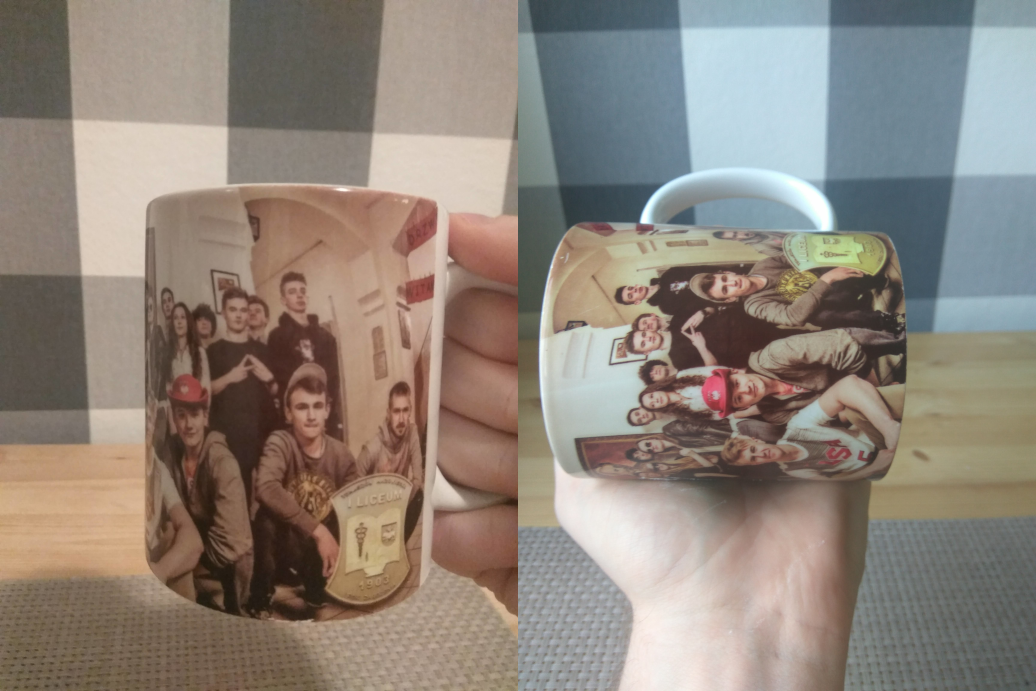
\includegraphics[width=7cm]{mug_clean_out}
    \end{minipage}%
    \begin{minipage}{.5\textwidth}
        \caption{Wynik badania spójności}
        \centering
        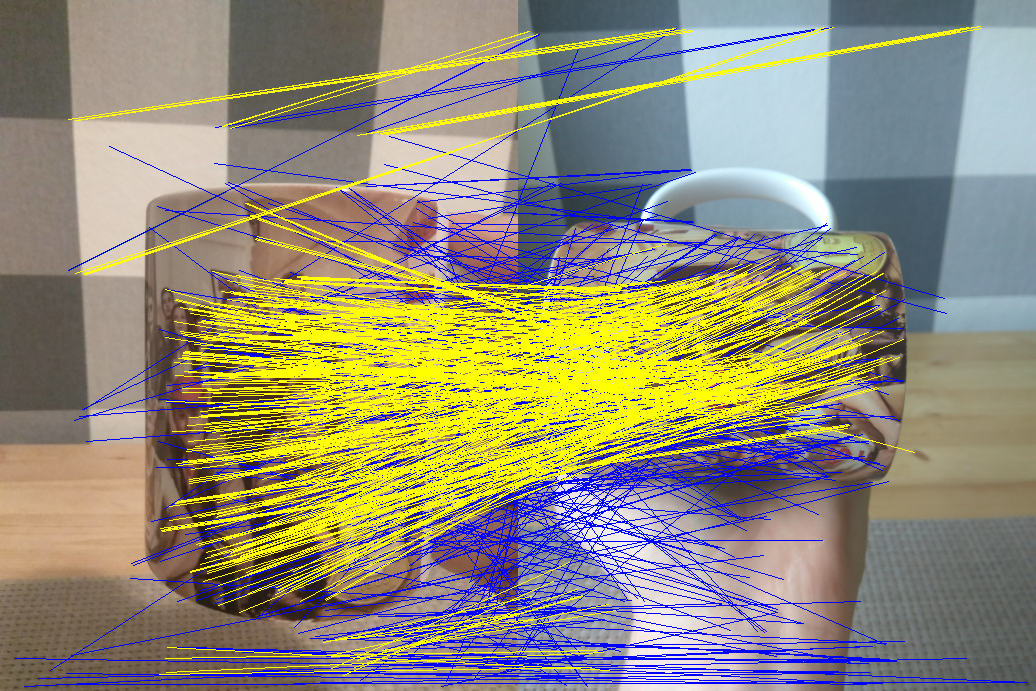
\includegraphics[width=7cm]{mug_pairs_conspairs_out}
    \end{minipage}%
    \end{figure}
    \begin{figure}[H]
    \centering
    \begin{minipage}{.5\textwidth}
        \caption{Wynik metody RANSAC}
        \centering
        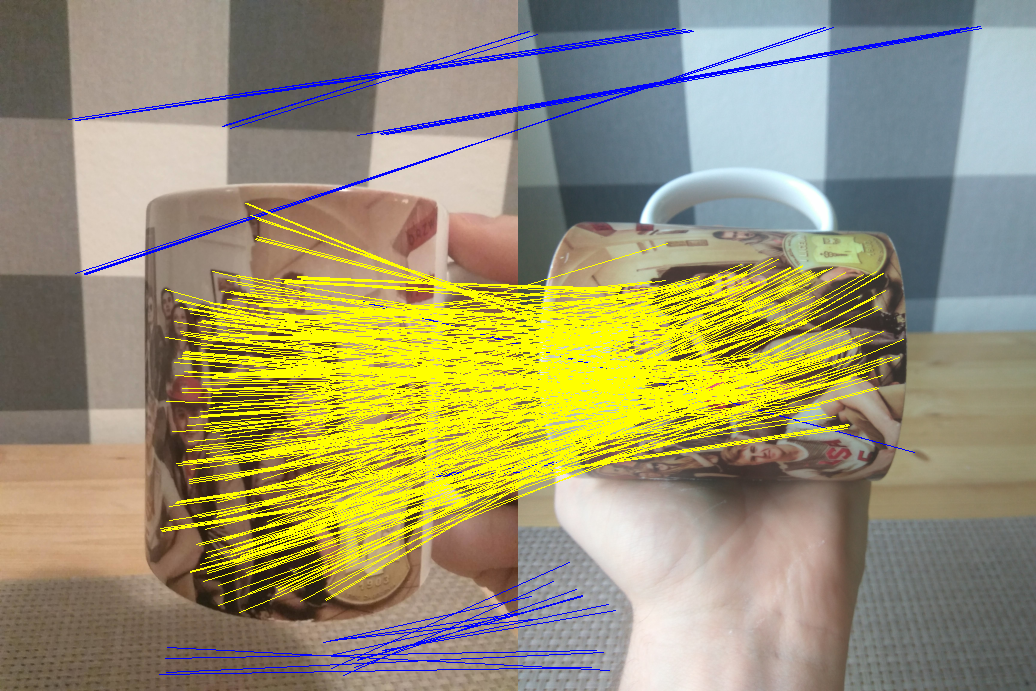
\includegraphics[width=7cm]{mug_pairs_ranscons_out}
    \end{minipage}%
    \begin{minipage}{.5\textwidth}
        \begin{table}[H]
        \caption{Zestawienie wyników par w etapach}
        \label{t:mug}
        \begin{center}
        \begin{tabular}{|c|c|c|c|c|} 
        \hline
        \thead{Punkty \\ (obraz 1)} & \thead{Punkty \\ (obraz 2)} & \thead{Pary \\ punktów} 
        & \thead{Pary \\ spójne} & \thead{Ostateczne \\ pary} \\
        \hline
        {3090} & {2821} & {758} & {451} & {410} \\
        \hline
        \end{tabular}
        \end{center}
        \end{table}
    \end{minipage}%
    \end{figure}
    
    \subsection{Portfel}
    W poniższym porównaniu zostały użyte dwa zdjęcia portfela w różnych sceneriach, na pierwszym zdjęciu portfel leży na blacie jest on trzymany w ręce. Dodatkowo zdjęcia zostały dokonane pod innym kątem i w różnej pozycji portfela. Niebieskie (ciemne)  linie oznaczają par punktów przed odfiltrowaniem (badanie spójności lub RANSAC), a żółte (jasne) po.
    
    \begin{figure}[H]
    \centering
    \begin{minipage}{.5\textwidth}
        \caption{Zdjęcia porównawcze}
        \centering
        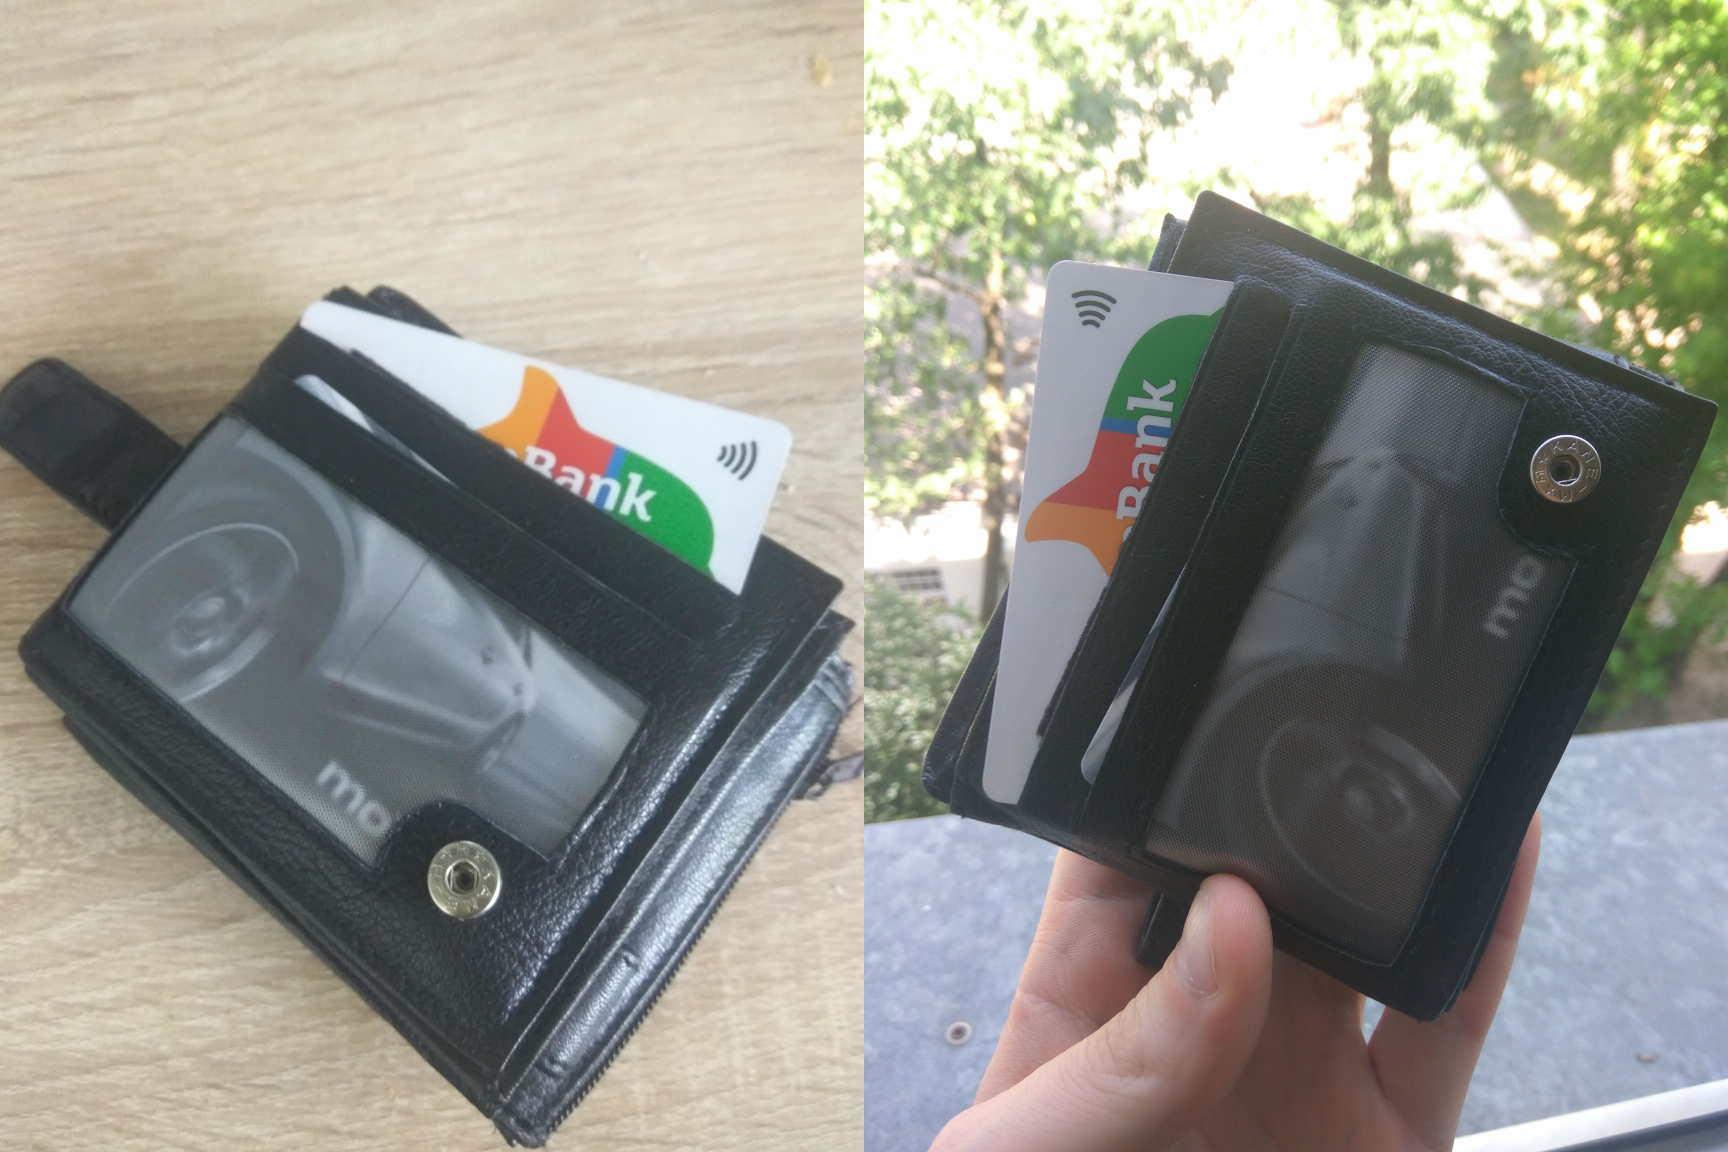
\includegraphics[width=7cm]{wallet_clean_out}
    \end{minipage}%
    \begin{minipage}{.5\textwidth}
        \caption{Wynik badania spójności}
        \centering
        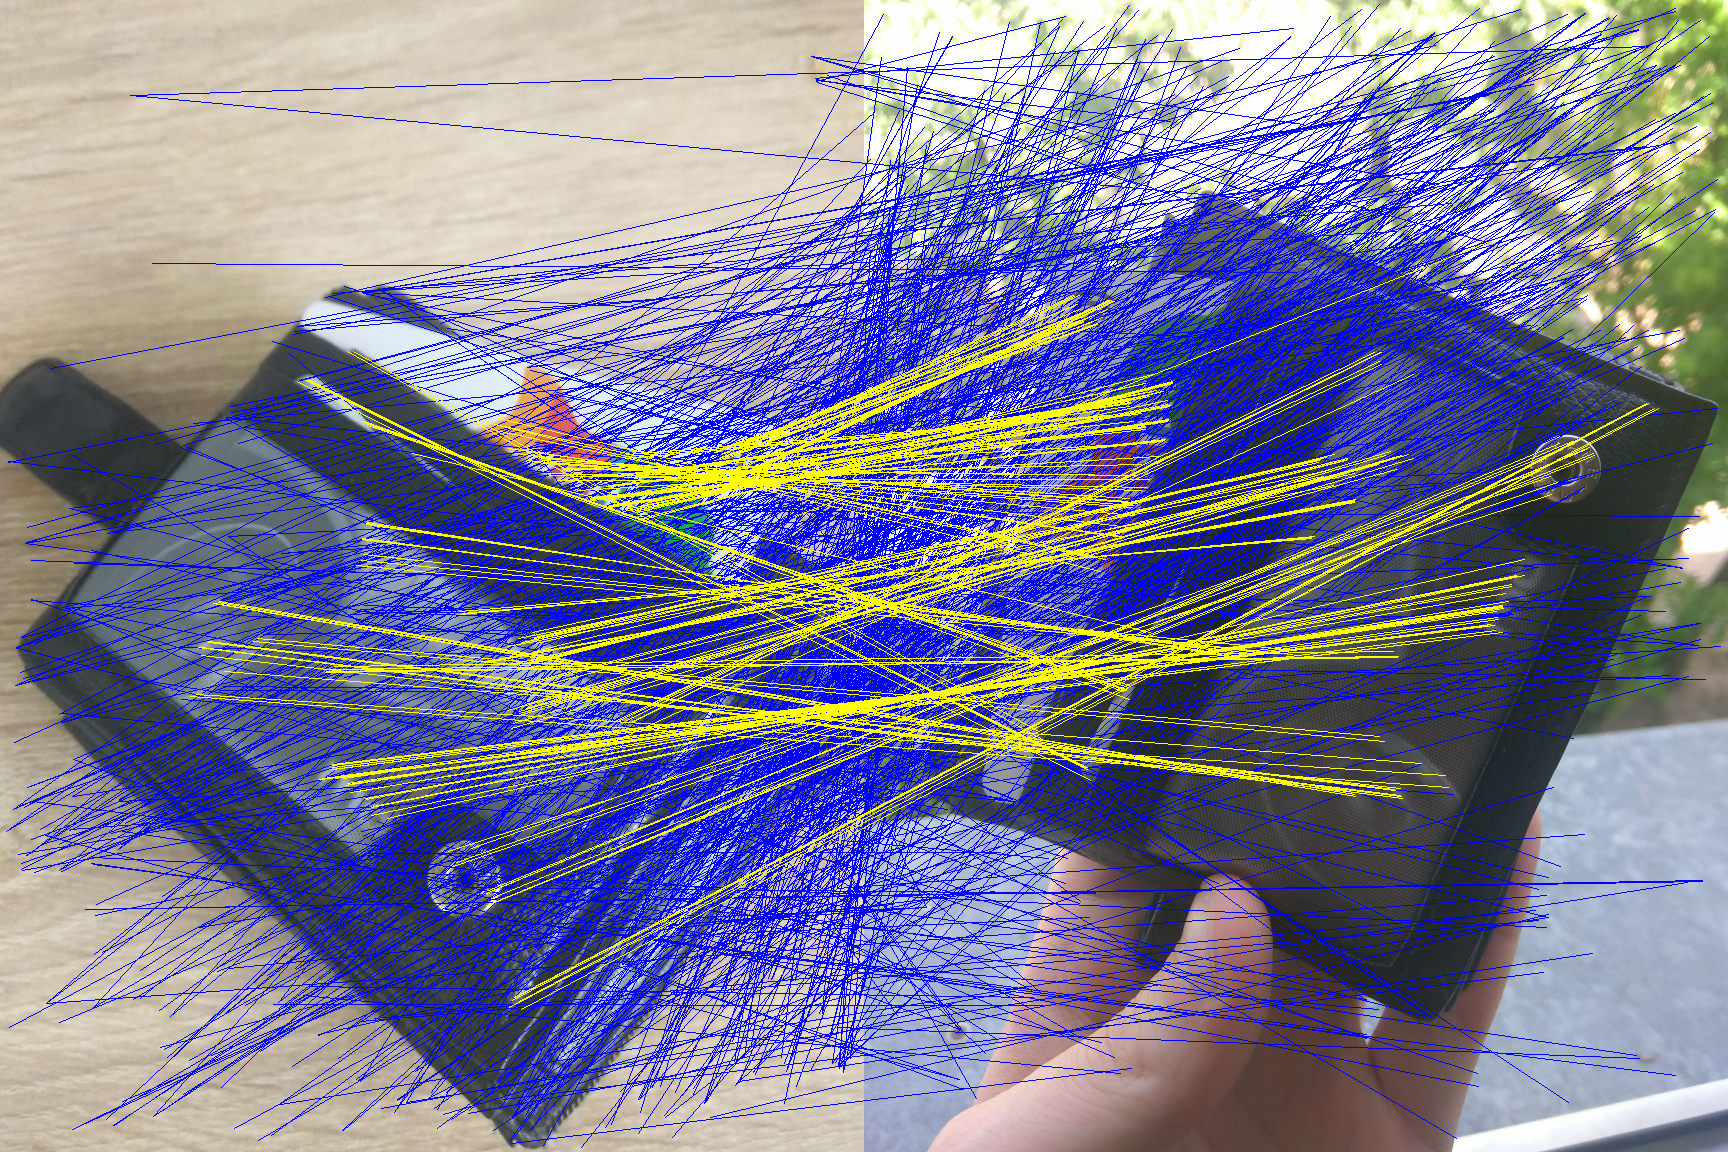
\includegraphics[width=7cm]{wallet_pairs_conspairs_out}
    \end{minipage}%
    \end{figure}
    \begin{figure}[H]
    \centering
    \begin{minipage}{.5\textwidth}
        \caption{Wynik metody RANSAC}
        \centering
        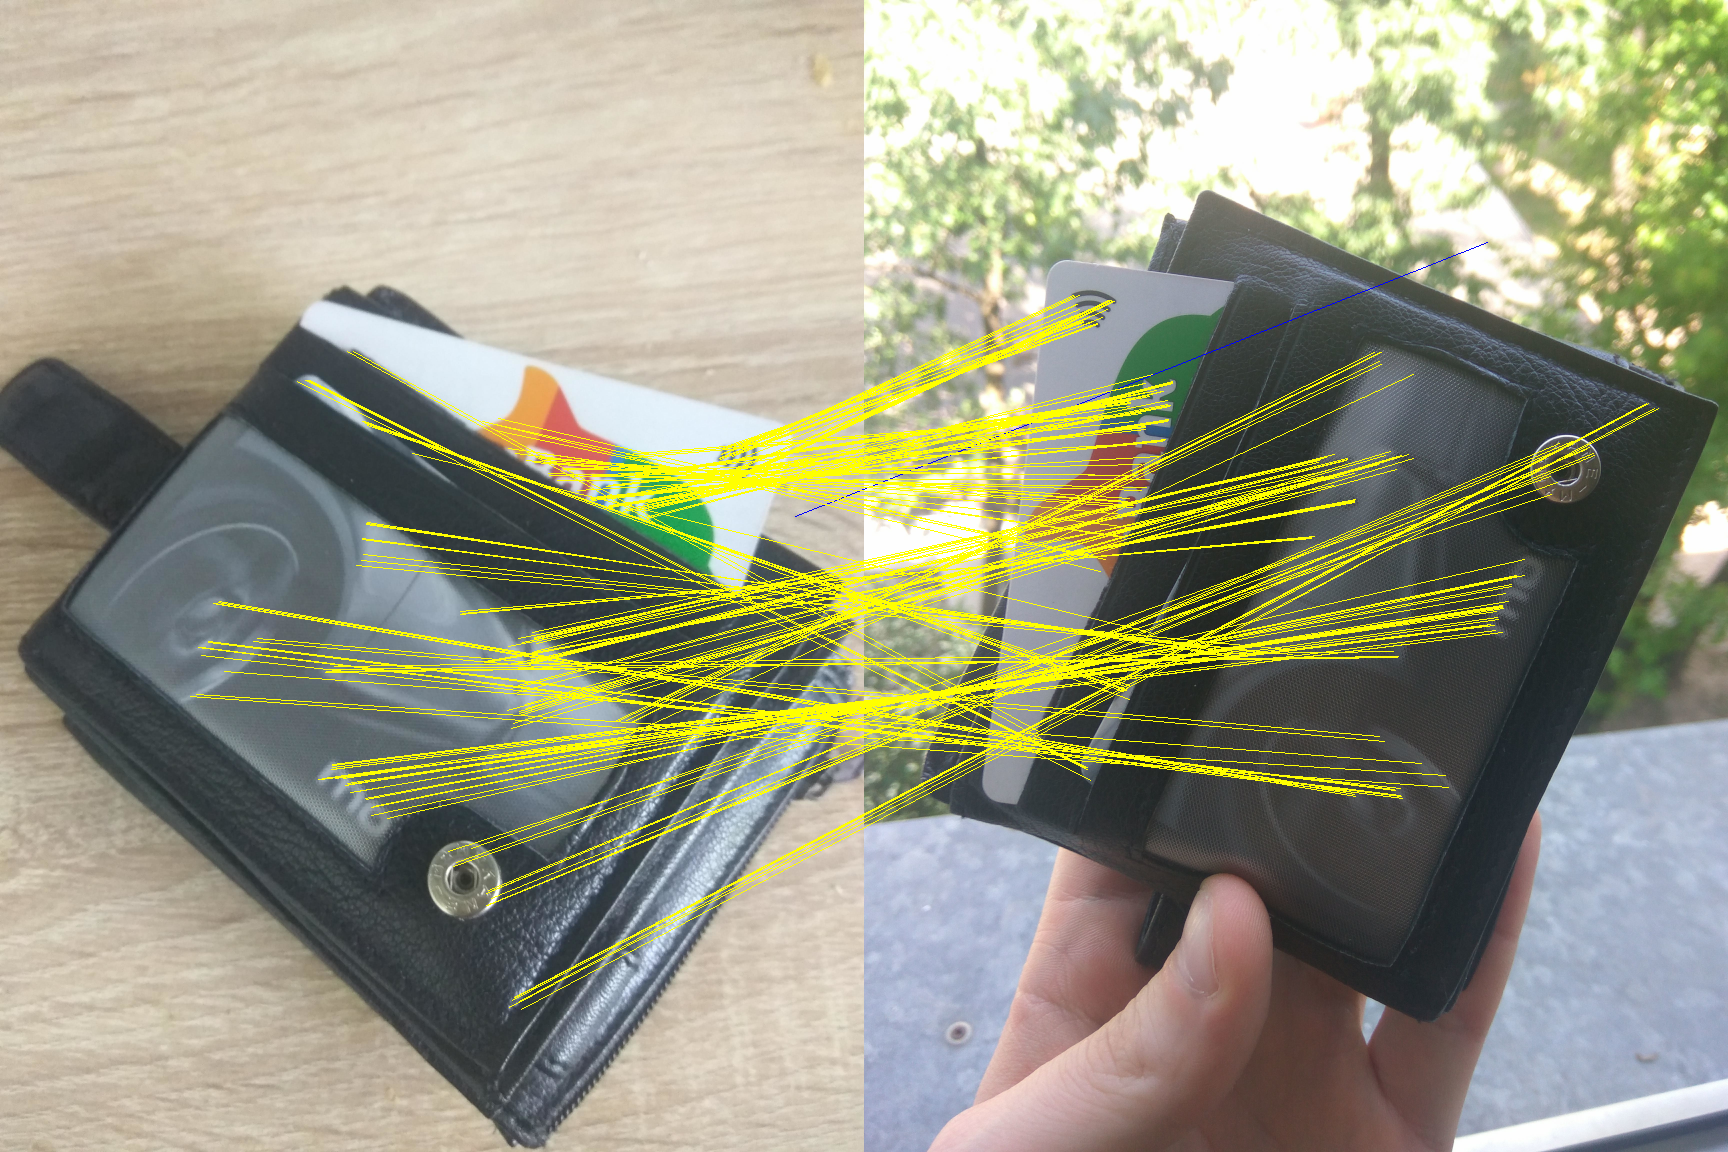
\includegraphics[width=7cm]{wallet_pairs_ranscons_out}
    \end{minipage}%
    \begin{minipage}{.5\textwidth}
            \begin{table}[H]
            \caption{Zestawienie wyników par w etapach}
            \label{t:wallet}
            \begin{center}
            \begin{tabular}{|c|c|c|c|c|} 
            \hline
            \thead{Punkty \\ (obraz 1)} & \thead{Punkty \\ (obraz 2)} & 
            \thead{Pary \\ punktów} & \thead{Pary \\ spójne} &
            \thead{Ostateczne \\ pary} \\
            \hline
            {3986} & {9905} & {1075} & {265} & {261} \\
            \hline
            \end{tabular}
            \end{center}
            \end{table}
    \end{minipage}%
    \end{figure}
    
    \subsection{Mysz komputerowa}
     Zdjęcia zostały zrobione z różnych odległości oraz pod lekko innym kątem, tło pozostało takie samo dlatego nadal występują pary łączące podkładkę zamiast myszki. Niebieskie (ciemne)  linie oznaczają par punktów przed odfiltrowaniem (badanie spójności lub RANSAC), a żółte (jasne) po.
    
    \begin{figure}[H]
    \centering
    \begin{minipage}{.5\textwidth}
        \caption{Zdjęcia porównawcze}
        \centering
        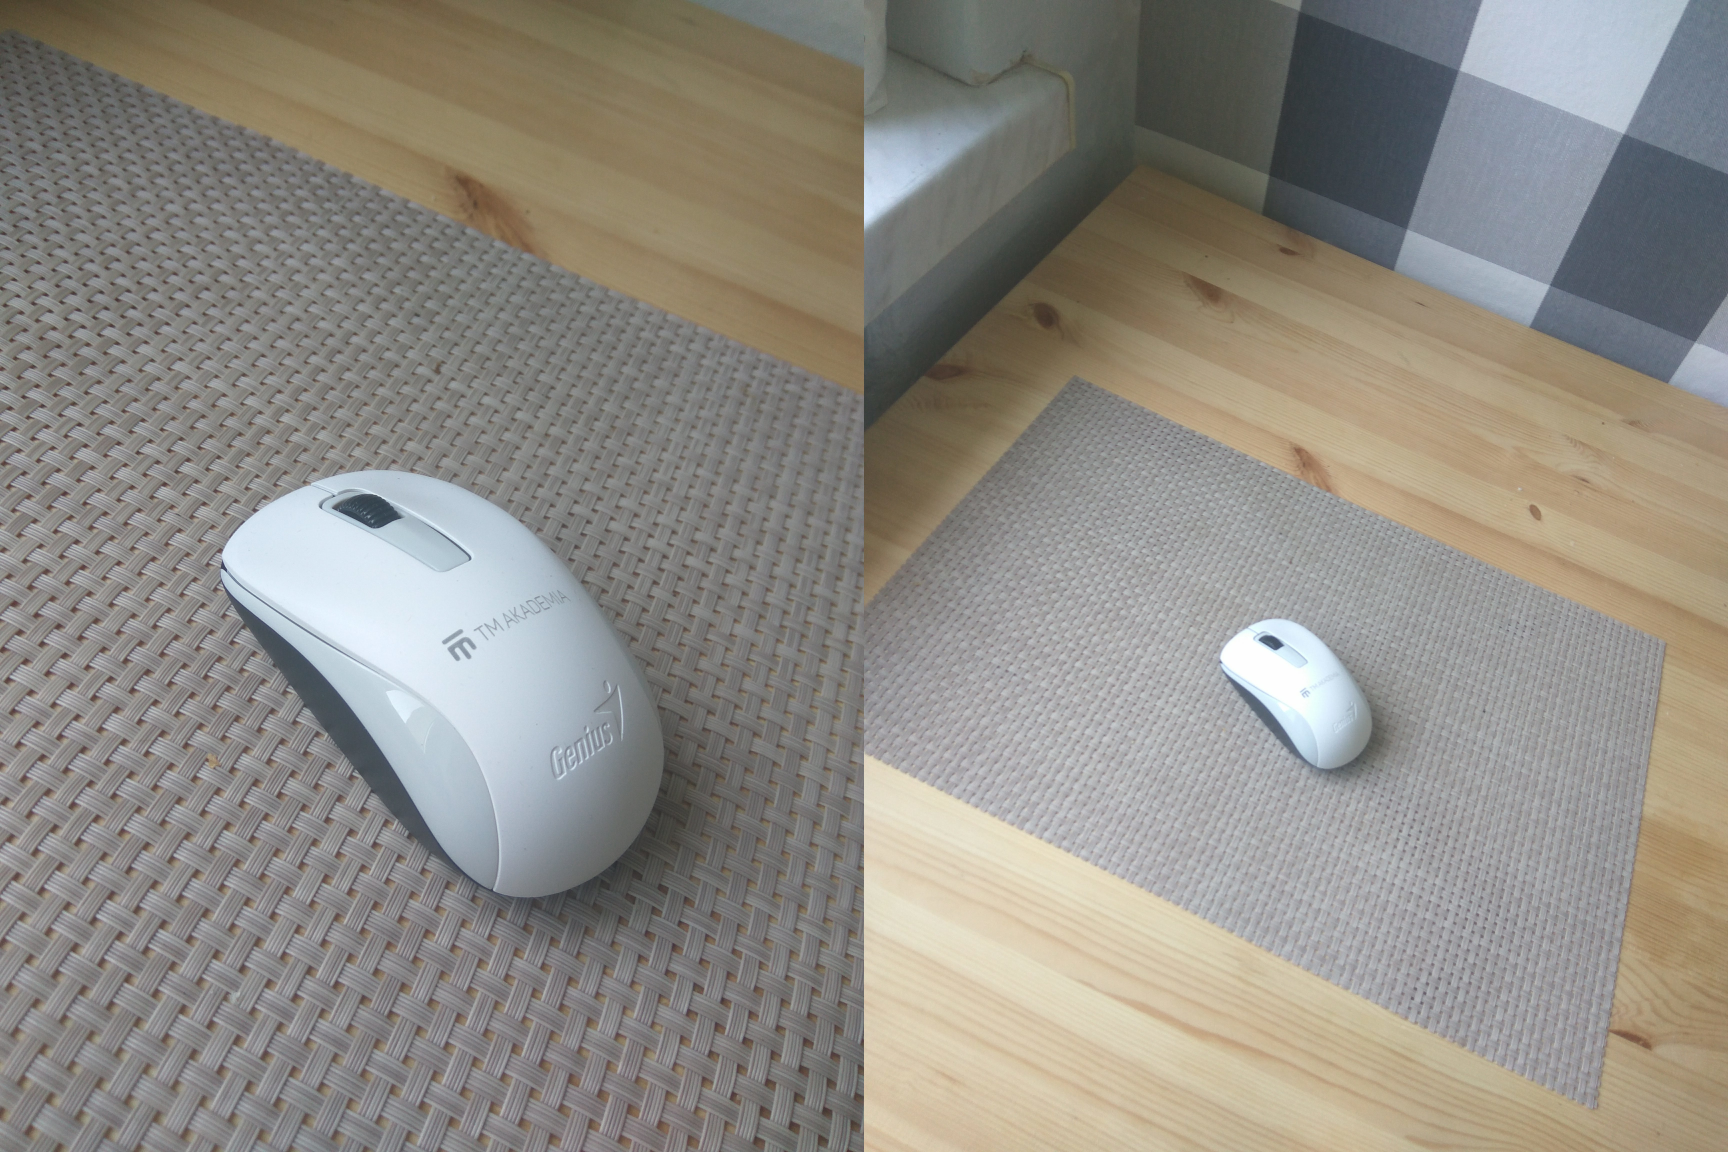
\includegraphics[width=7cm]{mouse_kitchen_clean_out}
    \end{minipage}%
    \begin{minipage}{.5\textwidth}
        \caption{Wynik badania spójności}
        \centering
        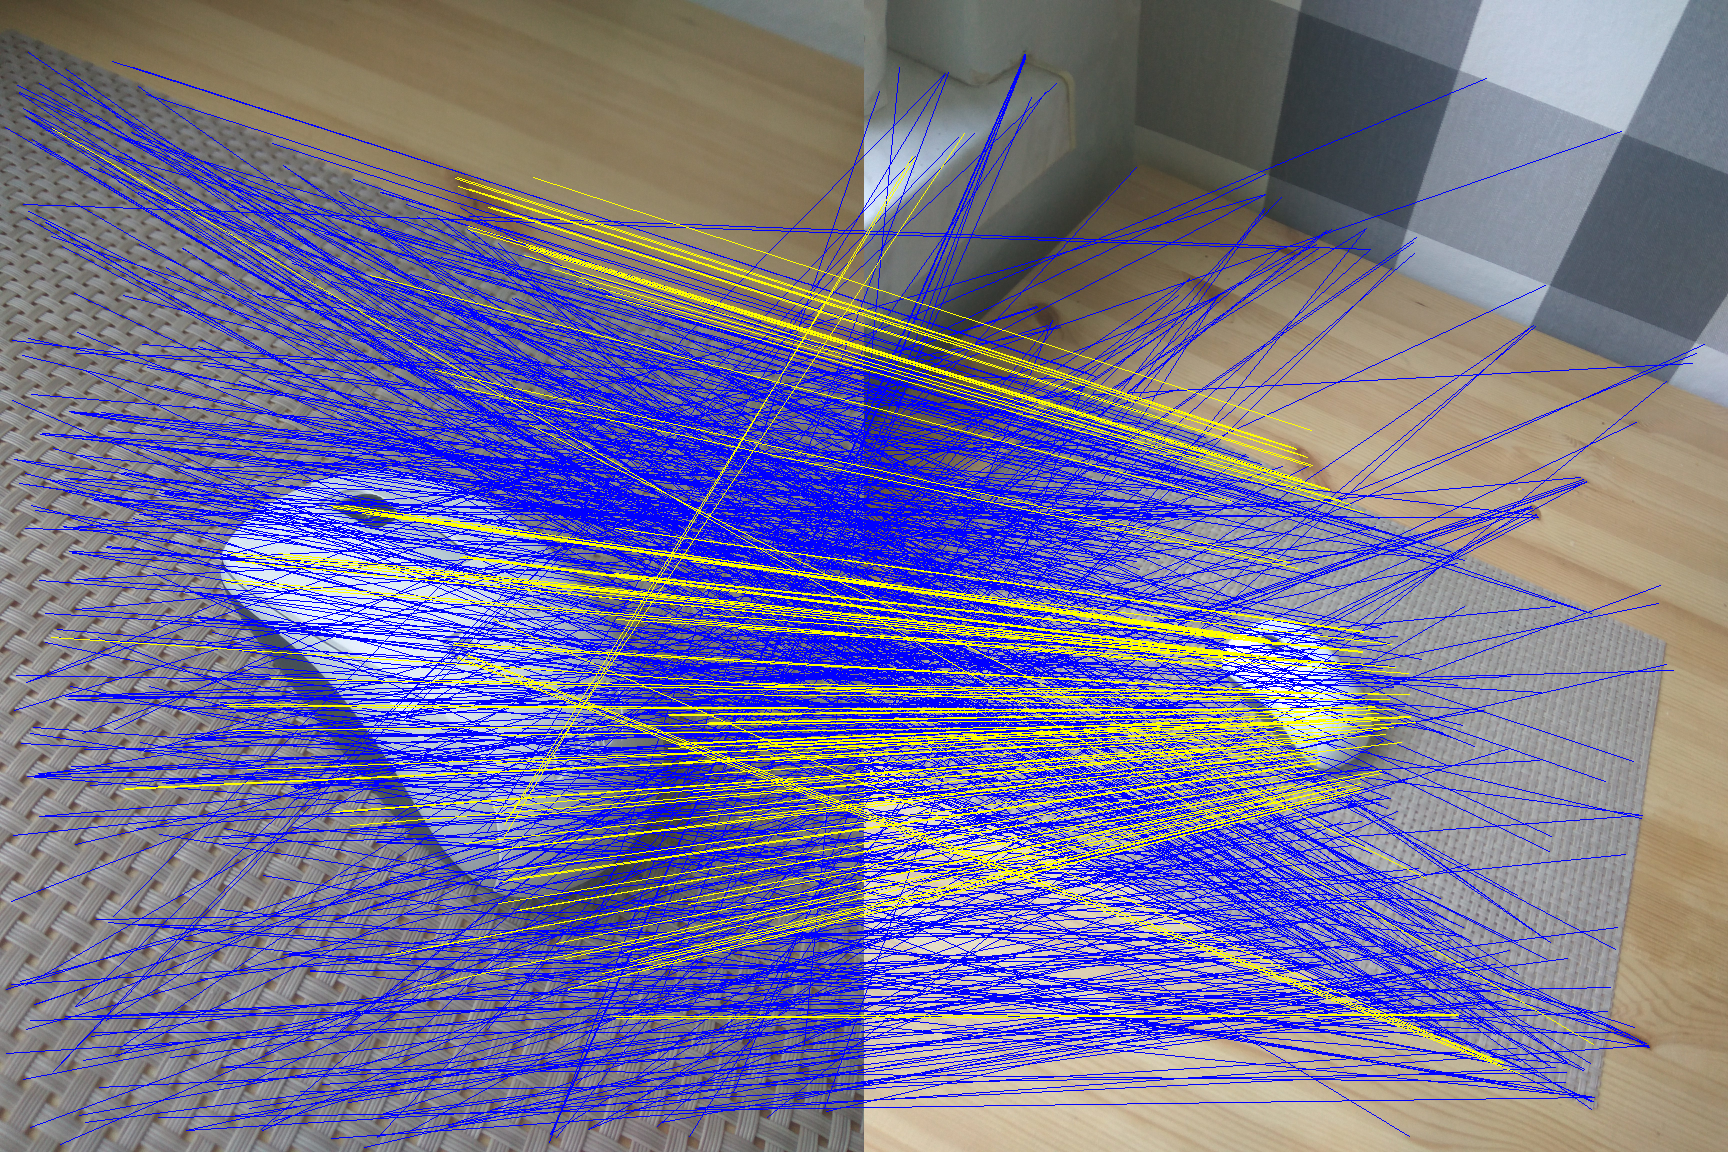
\includegraphics[width=7cm]{mouse_kitchen_pairs_conspairs_out}
    \end{minipage}%
    \end{figure}
    \begin{figure}[H]
    \centering
    \begin{minipage}{.5\textwidth}
        \caption{Wynik metody RANSAC}
        \centering
        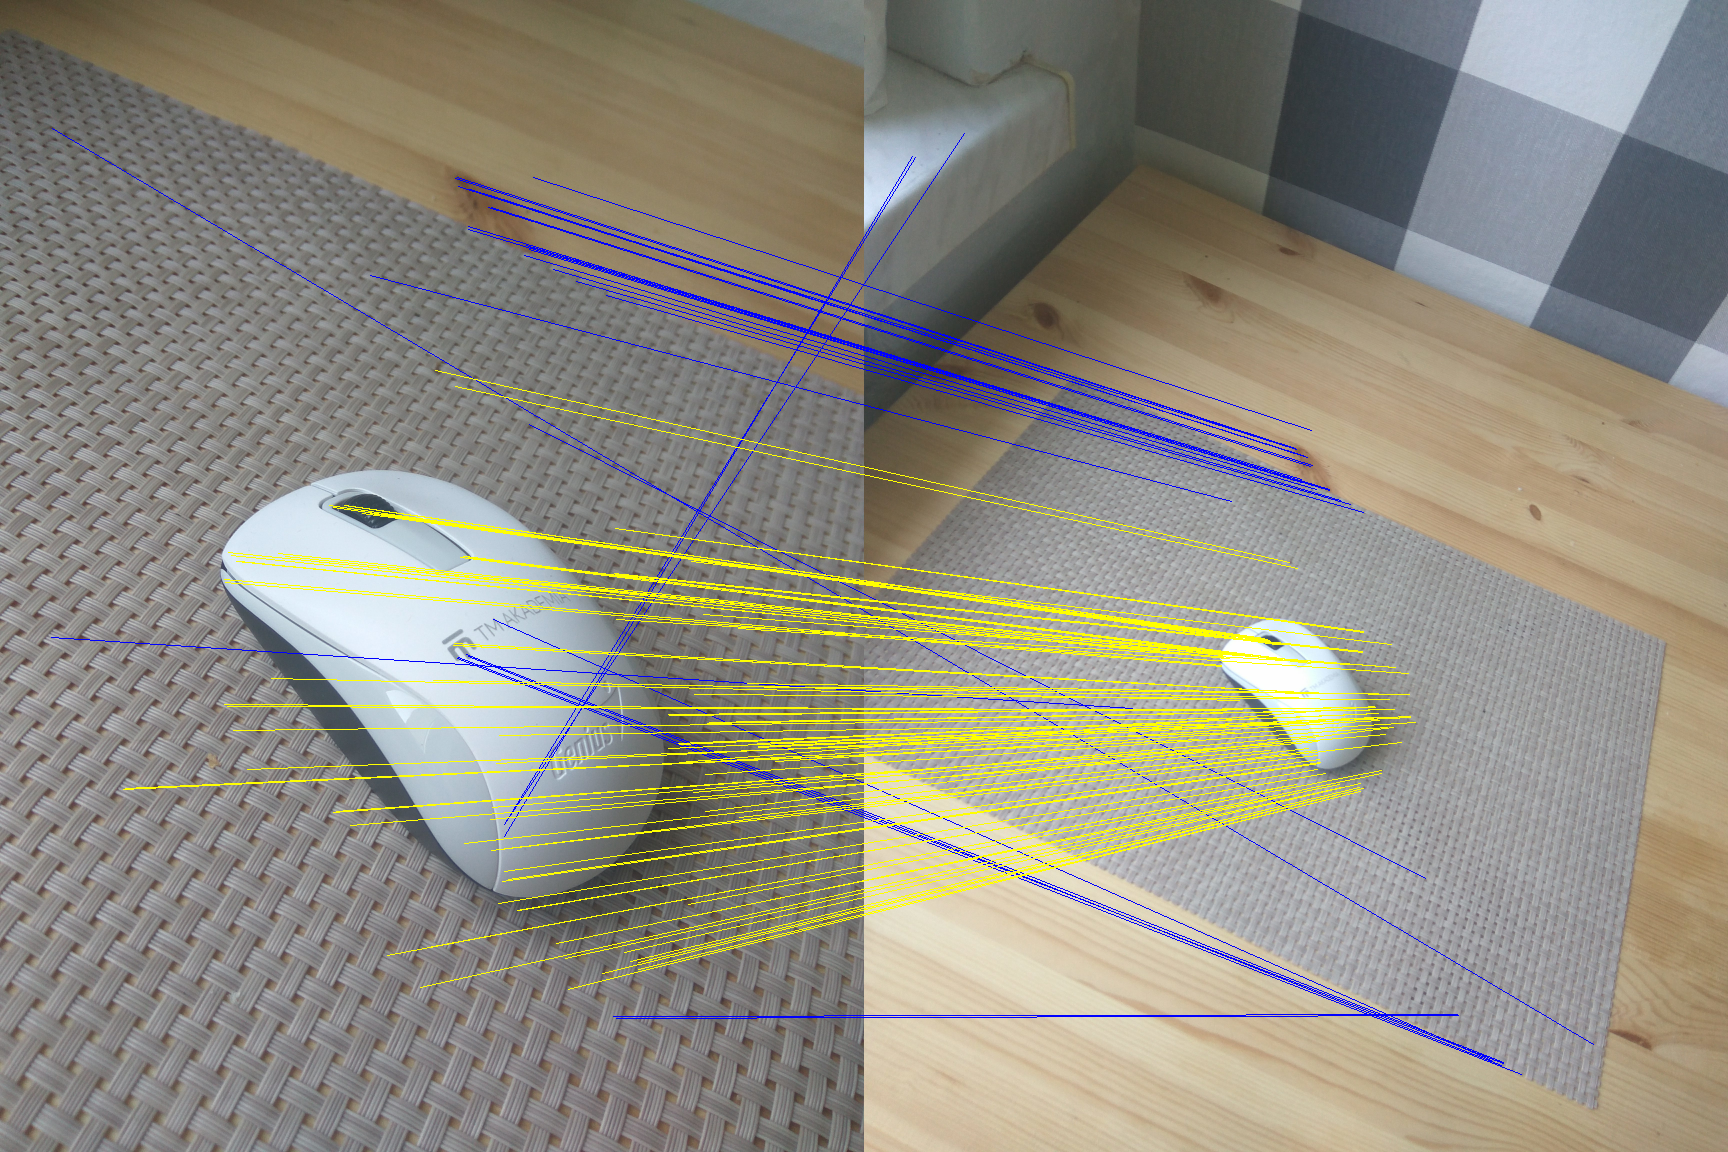
\includegraphics[width=7cm]{mouse_kitchen_pairs_ranscons_out}
    \end{minipage}%
    \begin{minipage}{.5\textwidth}
            \begin{table}[H]
            \caption{Zestawienie wyników par w etapach}
            \label{t:mouse}
            \begin{center}
            \begin{tabular}{|c|c|c|c|c|} 
            \hline
            \thead{Punkty \\ (obraz 1)} & \thead{Punkty \\ (obraz 2)} & \thead{Pary \\ punktów} & \thead{Pary \\ spójne} &
            \thead{Ostateczne \\ pary} \\
            \hline
            {15806} & {5939} & {851} & {149} & {112} \\
            \hline
            \end{tabular}
            \end{center}
            \end{table}
    \end{minipage}%
    \end{figure}

    
    \subsection{Książka}
    Zdjęcia książki zostały zrobione w różnej scenerii i pod różnymi kątami. Niebieskie (ciemne)  linie oznaczają par punktów przed odfiltrowaniem (badanie spójności lub RANSAC), a żółte (jasne) po.
    
    \begin{figure}[H]
    \centering
    \begin{minipage}{.5\textwidth}
        \caption{Zdjęcia porównawcze}
        \centering
        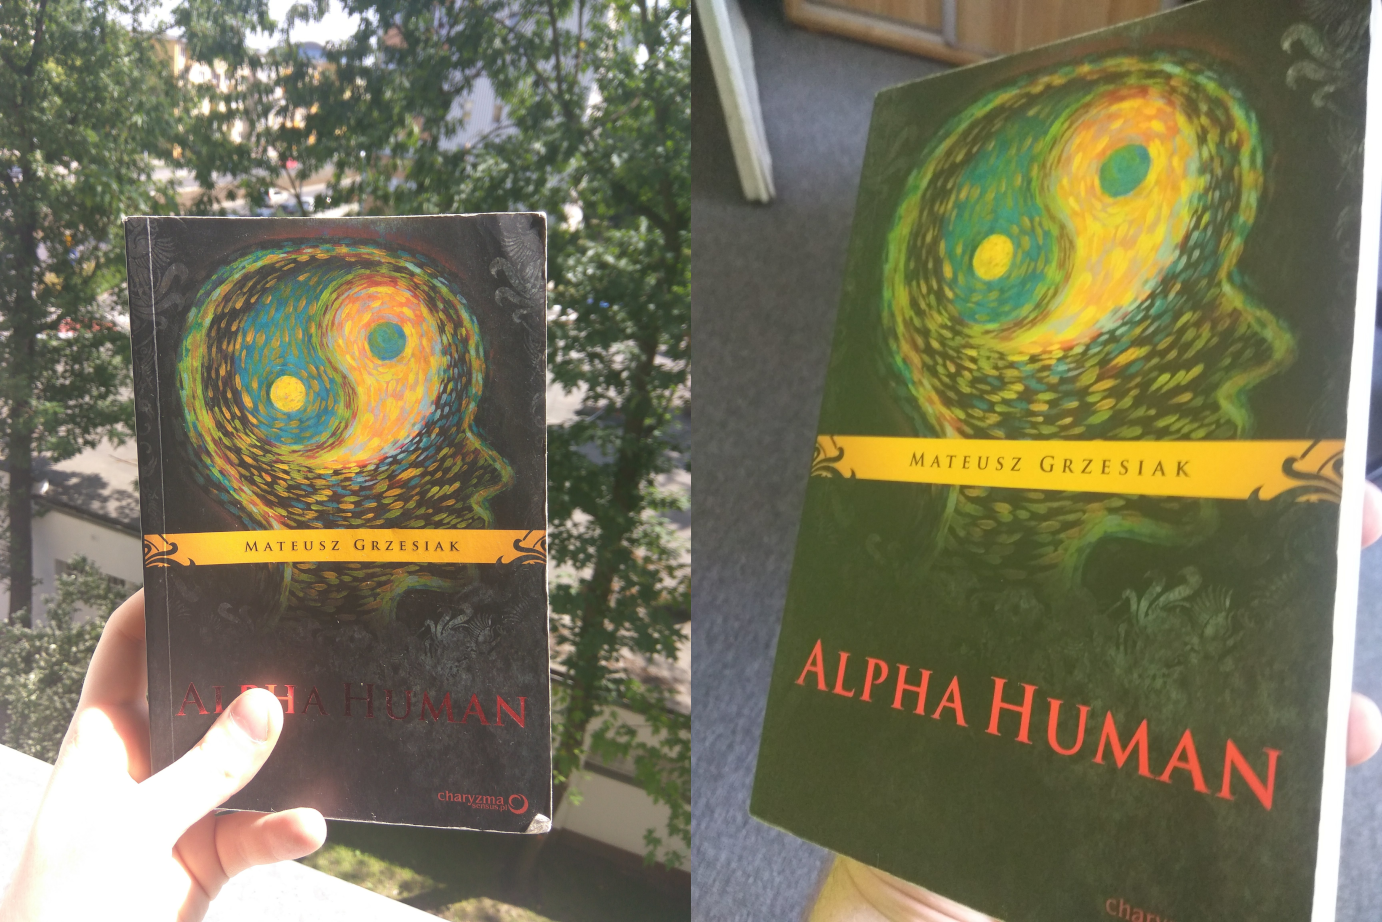
\includegraphics[width=7cm]{book__clean_out}
    \end{minipage}%
    \begin{minipage}{.5\textwidth}
        \caption{Wynik badania spójności}
        \centering
        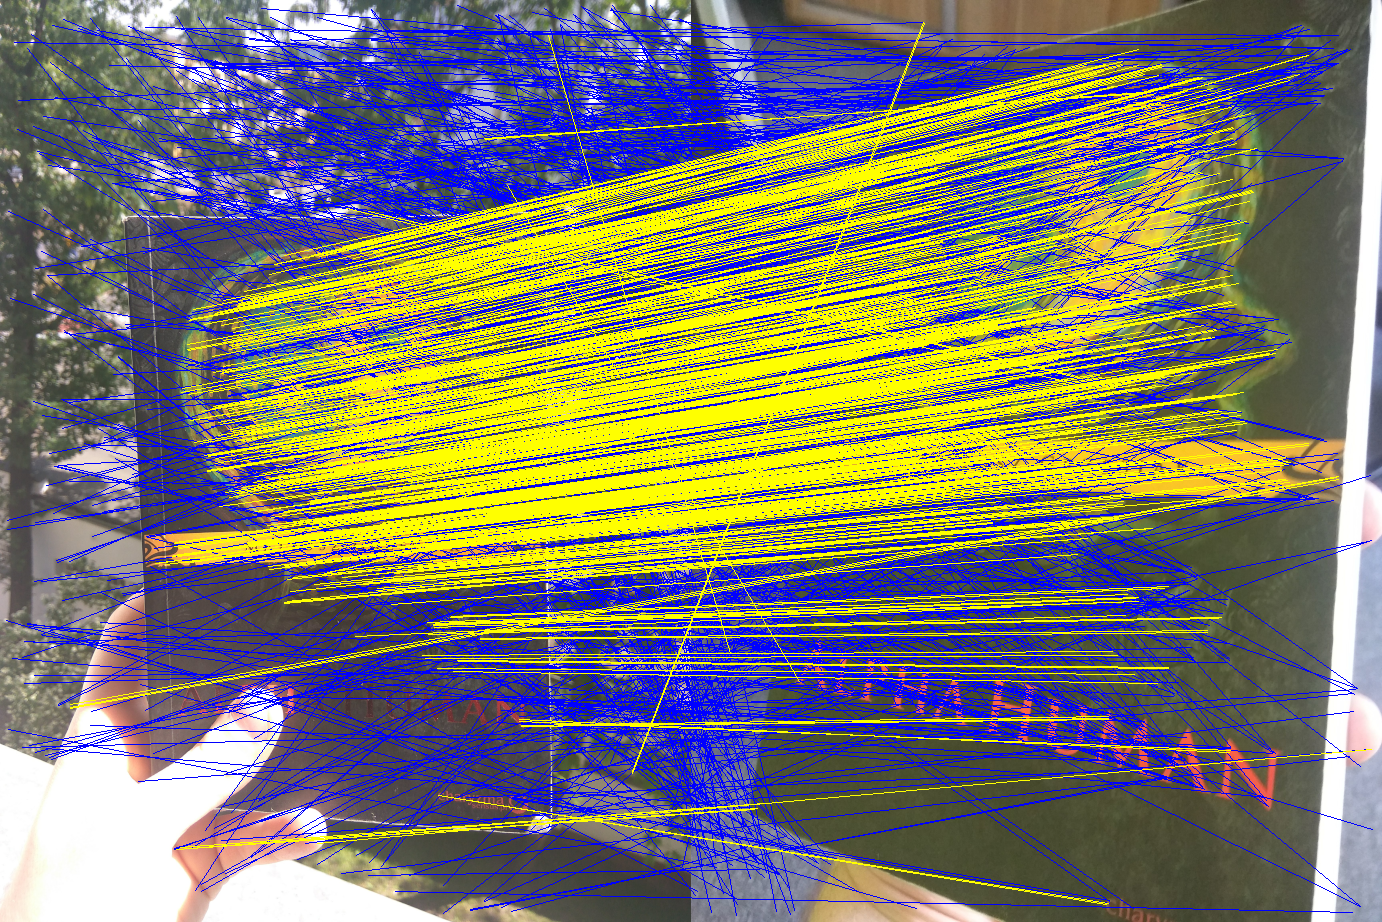
\includegraphics[width=7cm]{book__pairs_conspairs_out}
    \end{minipage}%
    \end{figure}
    \begin{figure}[H]
    \centering
    \begin{minipage}{.5\textwidth}
        \caption{Wynik metody RANSAC}
        \centering
        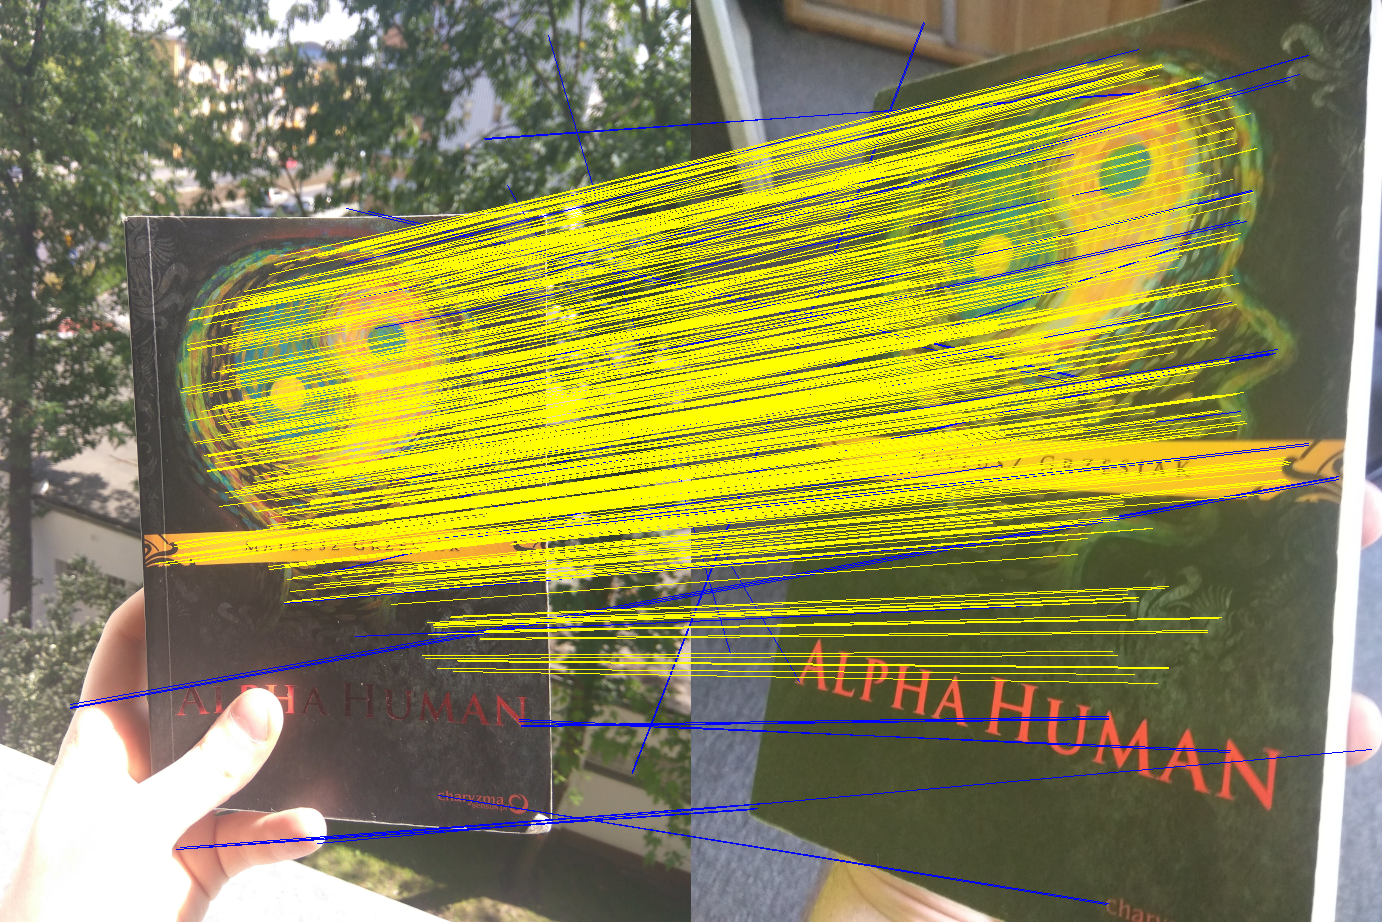
\includegraphics[width=7cm]{book__pairs_ranscons_out}
    \end{minipage}%
        \begin{minipage}{.5\textwidth}
                \begin{table}[H]
            \caption{Zestawienie wyników par w etapach}
            \label{t:book}
            \begin{center}
            \begin{tabular}{|c|c|c|c|c|} 
            \hline
            \thead{Punkty \\ (obraz 1)} & \thead{Punkty \\ (obraz 2)} & \thead{Pary \\ punktów} & \thead{Pary \\ spójne} &
            \thead{Ostateczne \\ pary} \\
            \hline
            {10654} & {5212} & {1548} & {717} & {647} \\
            \hline
            \end{tabular}
            \end{center}
            \end{table}
    \end{minipage}%
    \end{figure}
    
    \subsection{Kaktus}
    Zdjęcia zostały zrobione w różnych pomieszczeniach i odrobinę różnym oświetleniu. Niebieskie (ciemne)  linie oznaczają par punktów przed odfiltrowaniem (badanie spójności lub RANSAC), a żółte (jasne) po.
    W przypadku tej pary zdjęć konieczne była modyfikacja parametrów algorytmu spójności sąsiedztwa, liczba sąsiadów została zredukowana do 10, natomiast próg spójności został zmniejszony do wartości 0.35. W przypadku większych parametrów algorytm nie potrafił znaleźć żadnej pary punktów spójnych.
    
    \begin{figure}[H]
    \centering
    \begin{minipage}{.5\textwidth}
        \caption{Zdjęcia porównawcze}
        \centering
        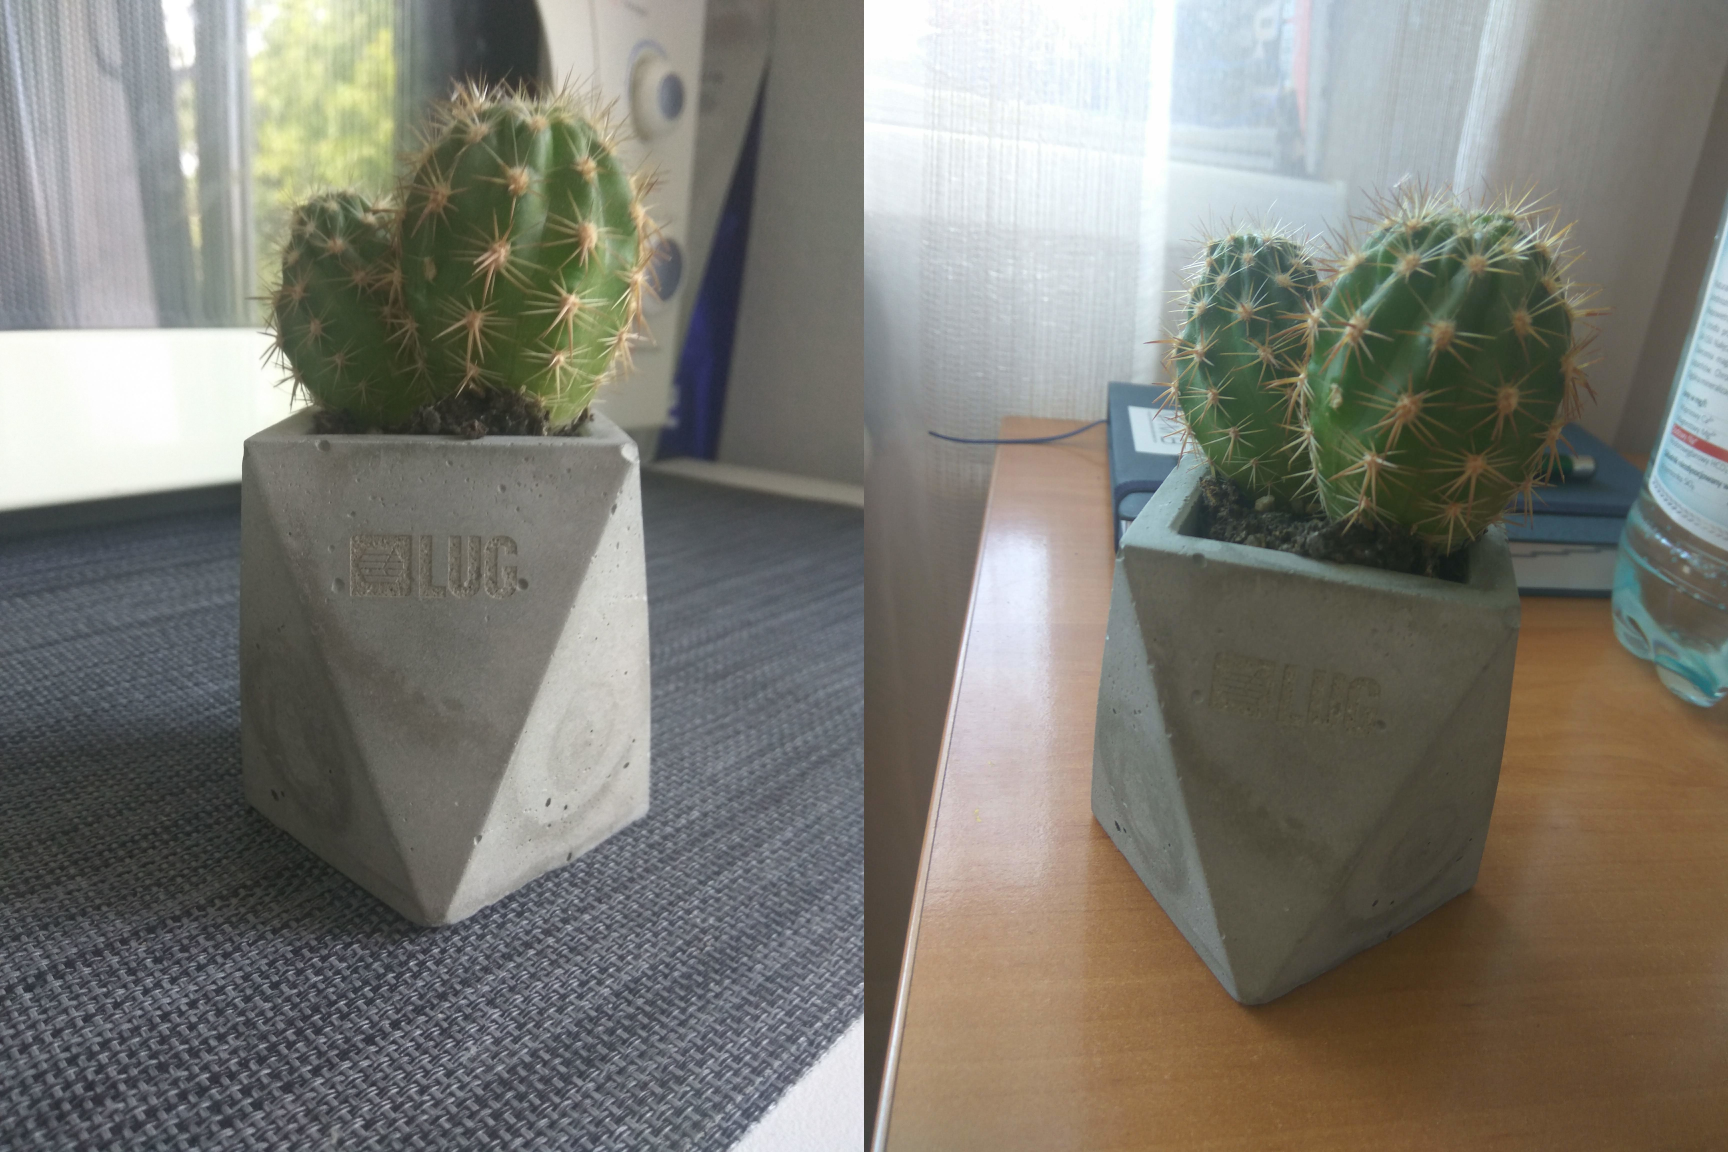
\includegraphics[width=7cm]{cactus_clean_out}
    \end{minipage}%
    \begin{minipage}{.5\textwidth}
        \caption{Wynik badania spójności}
% %         \centering
        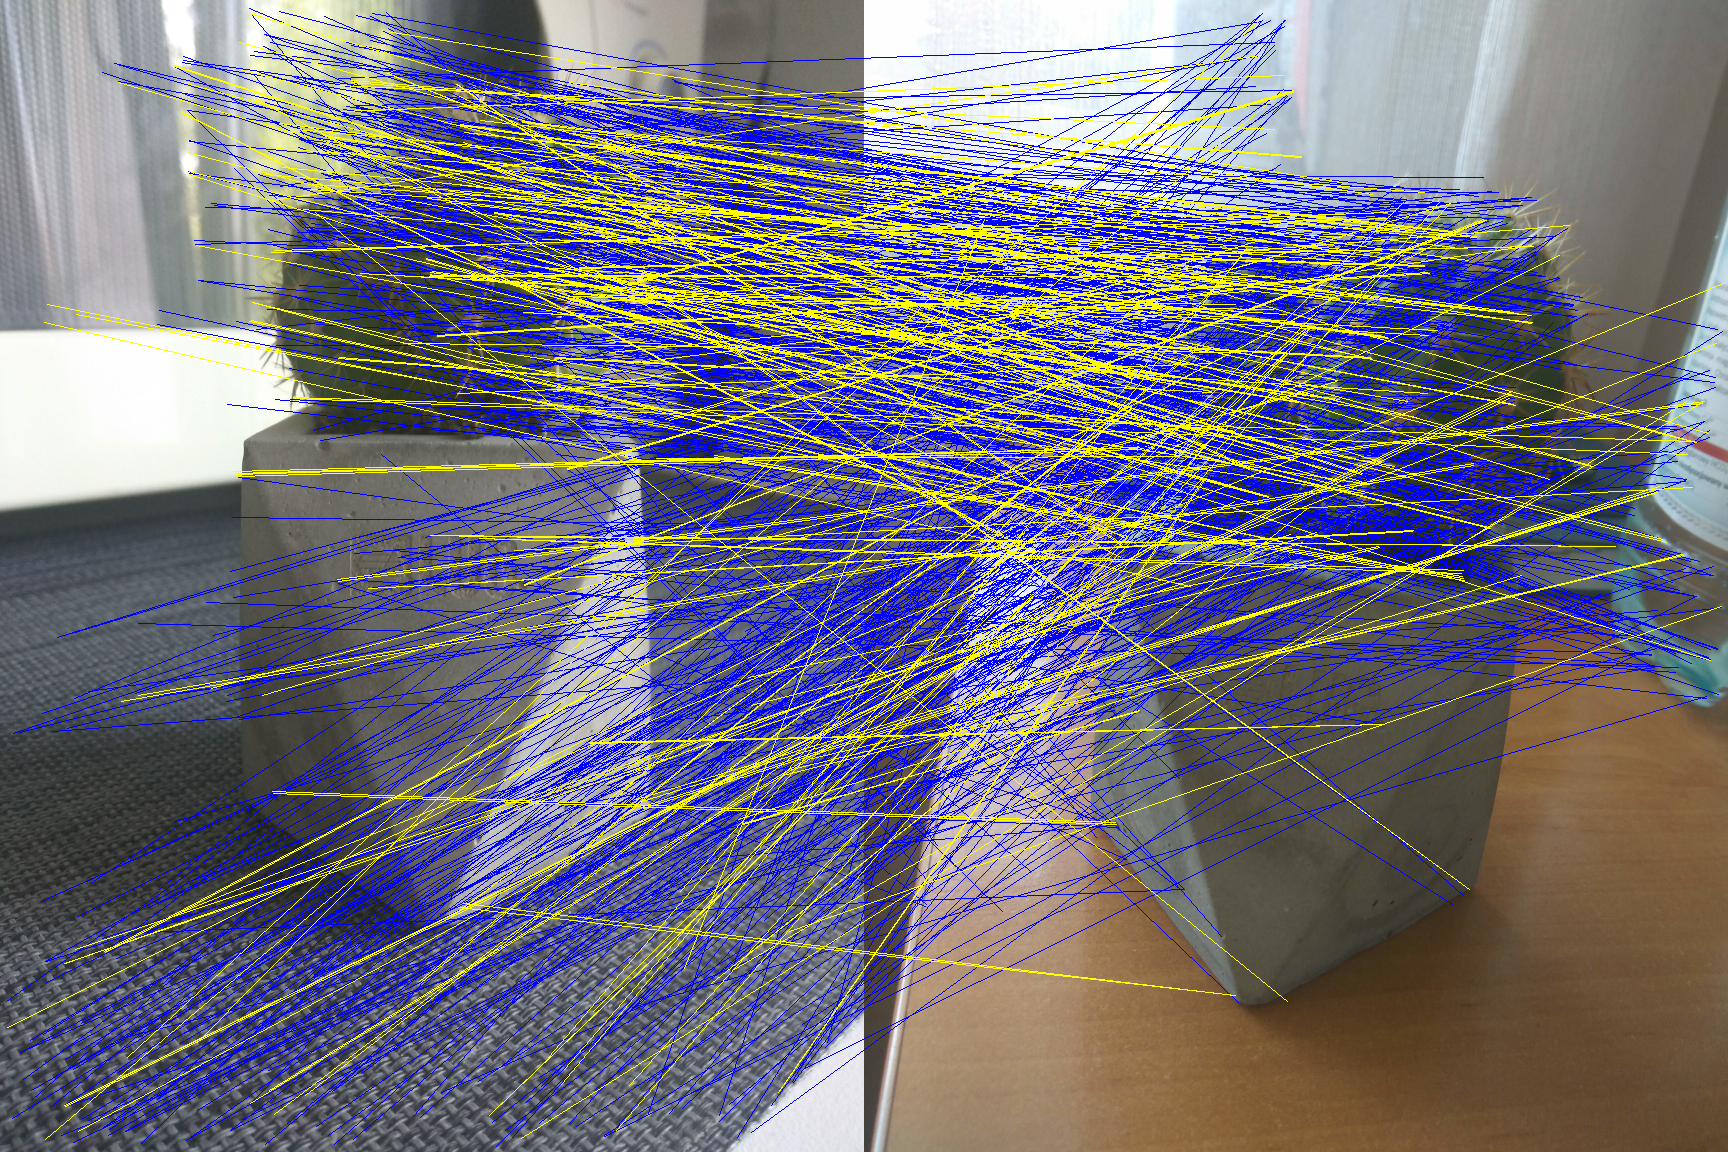
\includegraphics[width=7cm]{cactus_pairs_conspairs_out}
    \end{minipage}%
    \end{figure}
    \begin{figure}[H]
    \centering
    \begin{minipage}{.5\textwidth}
        \caption{Wynik metody RANSAC}
        \centering
        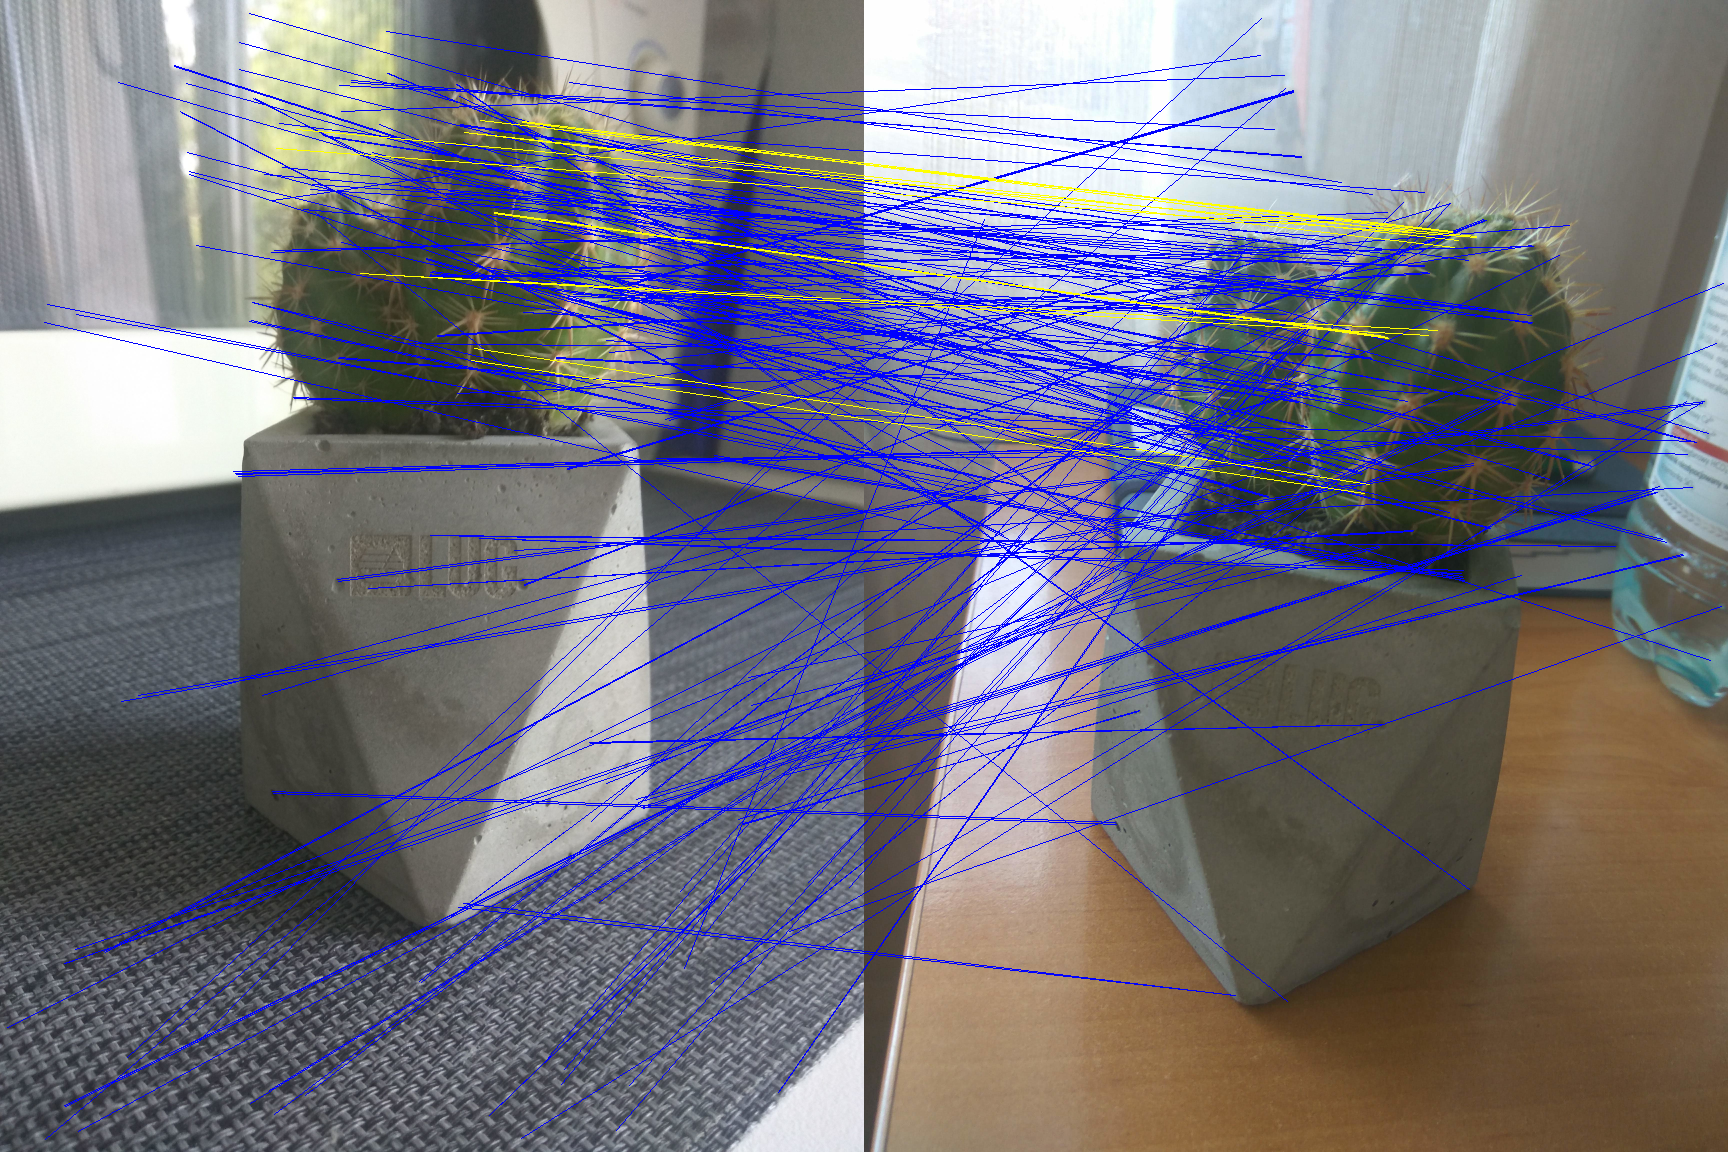
\includegraphics[width=7cm]{cactus_pairs_ranscons_out}
    \end{minipage}%
    \begin{minipage}{.5\textwidth}
        \begin{table}[H]
        \caption{Zestawienie wyników par w etapach}
        \label{t:cactus}
        \begin{center}
        \begin{tabular}{|c|c|c|c|c|} 
        \hline
        \thead{Punkty \\ (obraz 1)} & \thead{Punkty \\ (obraz 2)} & \thead{Pary \\ punktów} & \thead{Pary \\ spójne} &
        \thead{Ostateczne \\ pary} \\
        \hline
        {12967} & {3569} & {946} & {90} & {18} \\
        \hline
        \end{tabular}
        \end{center}
        \end{table}
    \end{minipage}%
    \end{figure}
    
    \justify
    \subsection{Omówienie wyników}
    Wynik w przypadku większości badanych par obrazów jest zadowalający, widoczna jest redukcja par zarówno po sprawdzeniu spójności jak i uruchomieniu metody RANSAC. Najlepsze rezultaty uzyskano podczas badania zdjęć kubka oraz książki. W przypadku myszki i kaktusa skrypt wyznaczający punkty kluczowe skupiał się nie na samym przedmiocie, a powierzchni na której leżały przedmioty. Z tego powodu liczba par spójnych była bardzo mała w stosunku do liczby punktów kluczowych na obu obrazach i została ponownie zredukowana po użyciu metody RANSAC. Pary punktów kluczowych były wyznaczane na podstawie błędu średniokwadratowego z cech punktów, być może inna metoda pozwoliłaby na uzyskanie lepszych rezultatów. Liczba spójnych par mogłaby także zostać zwiększona poprzez obniżenie progu spójności, który w przypadku badanych obrazów wynosił 0.4.
 
\end{document}
